\section{Attack Model}
\label{sec:attack}
\begin{figure*}[h]
	\centering
	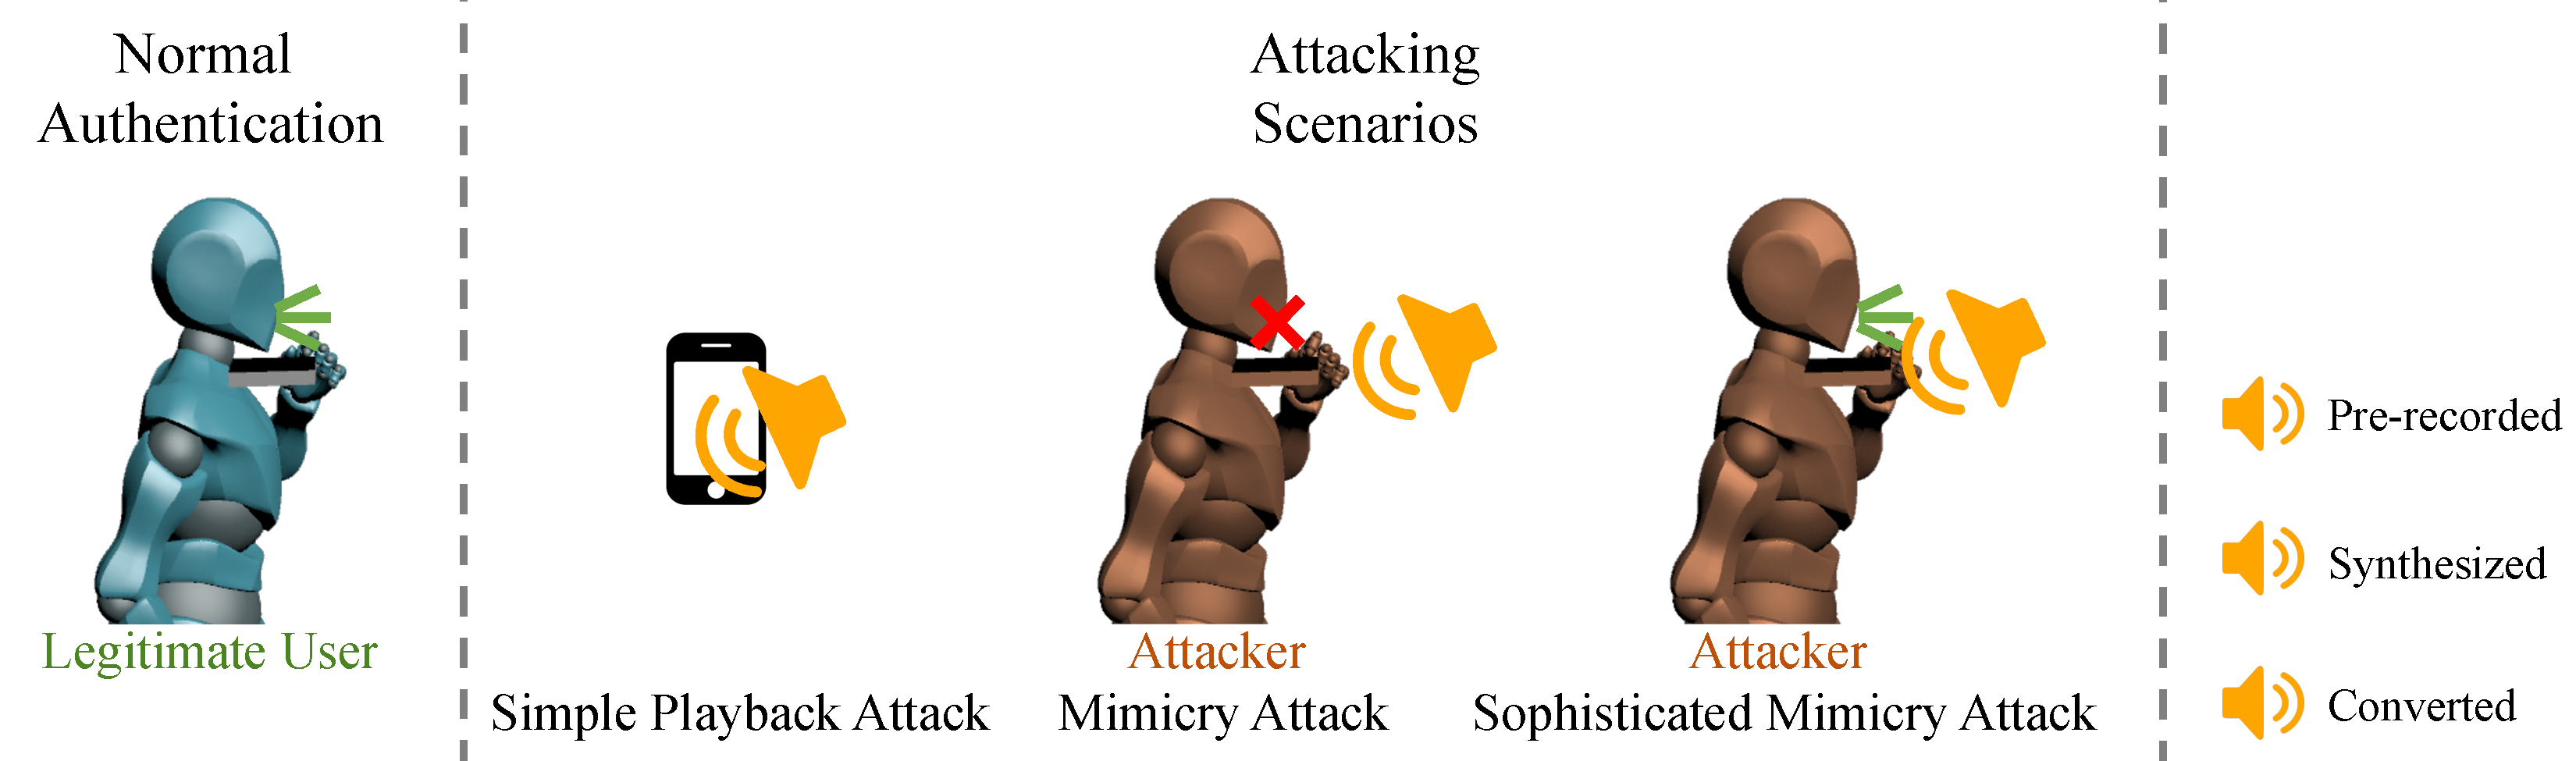
\includegraphics[width=.9\linewidth]{attack}
	\caption[MoVo Attack Model]{Attack Model: There are three types of attack scenarios. To conduct a simple playback attack, the target phone is placed in contact with the electronic speaker. To conduct a mimicry attack, the target phone is placed on the attacker's throat, but the attacker will not speak during the authentication period. As for a sophisticated mimicry attack, the attacker would try to mimic the victim's voice while playing the victim's sounds through electronic speakers. In the two mimicry attacking scenarios, the target phone is also in contact with the electronic speaker. In all three scenarios, the sound played by the electronic speaker could be the pre-recorded sound from the legitimate user, synthesized sound, or converted sound.}
	\label{fig:attack}
\end{figure*}


As mentioned in Section~\ref{sec:spoof}, traditional attacks to voice authentication are impersonation attacks, replay attacks, speech synthesis attacks, and voice conversion attacks. 
%
Real person impersonation attacks can be effectively defended by existing speaker recognition algorithms in general. For the other three, attackers acquire the legitimate user's voice samples either in place or online. The attacker then processes the samples in three ways to perform attacks: replay attack - concatenate voice segments to match the legitimate user's passphrase followed by harmful action or commands; speech synthesis - build speaker model and synthesize passphrase from texts; voice conversion - the attacker says the passphrase, then by spectral mapping and prosody conversion, the signals are manipulated to sound like the legitimate user's. 

If the attacker directly plays the processed sound signals through the speaker, he is conducting the \textit{simple playback attack}, no matter the processed signals are pre-recorded (replay attack), synthesized (speech synthesis), or converted (voice conversion).

A stronger attacker would perform the \textit{mimicry attack}, where the processed signals are still played by electronic speakers, but the attacker also needs to place the smartphone on his throat. In this case, the attacker can observe how the legitimate user passes the authentication\footnote{{\shortname} is a spoof-proof voice authentication system and require users to place the phone on the throat. For best user experience, it can downgrade to a normal voice authentication system and only process microphone data for normal use. Only when the user accesses sensitive information or makes dangerous operation, the spoof-proof mechanism will be invoked and the motion sensor would be in use.} and try to mimic the throat movement of the legitimate user. Note that we do not consider that the attacker uses the built-in speaker of the smartphone to play the processed signal, because if the attacker can control the built-in speaker, he has already hacked the targeted smartphone, which means there is no use to do voice authentication anymore. Therefore, the speaker, shown as yellow icons in Fig.~\ref{fig:attack} must be a different device from the smartphone.


The strongest attack is the \textit{sophisticated mimicry attack}, where the attacker would not only mimic the sound by the electronic device, but also by himself. Compared to the previous case, the attacker would speak the same word along while the electronic speaker is playing. Recall that impersonate the victim's voice using vocal organs is very hard, the attacker should either be professional impersonators or have natural voices similar to the victim's. Such a condition is hard to be met. Therefore, in this thesis, the sophisticated mimicry attacker only controls the timing (starting or pausing when speaking), but not timbre.

Note that we consider two mimicry attacks because these two have different emphasis: the 
mimicry attack makes sure the motion sensor data are affected by the victim's sound, while the sophisticated mimicry attack tries to add ``liveness'' to the motion sensor data. 
